
%(BEGIN_QUESTION)
% Copyright 2006, Tony R. Kuphaldt, released under the Creative Commons Attribution License (v 1.0)
% This means you may do almost anything with this work of mine, so long as you give me proper credit

Shown here is a typical set of ``curves'' for an overload heater, such as is commonly used to provide overcurrent protection for AC electric motors:

$$\includegraphics[width=15.5cm]{i02308x01.eps}$$

Why is there any time required to re-set an overload heater contact after a ``trip?''  Circuit breakers can be re-closed mere moments after a trip with no problem, and fuses (of course) can be replaced moments after blowing.  Is this an intentional design feature of overload heaters, or just an idiosyncrasy?

Also, explain why the reset curve starts to decrease for currents above 300\% of the motor's full-load rating.  Why doesn't the reset time curve continue to increase with increasing fault current magnitudes?

\underbar{file i02308}
%(END_QUESTION)





%(BEGIN_ANSWER)

The reset time for an overcurrent heater is an intentional design feature.  If the heater is too hot to re-set, then the motor is too hot to re-start.

\vskip 10pt

Remember that the purpose of an overload heater is to provide a {\it thermal analogue} of the electric motor itself.  Ideally, the heater heats up and cools down at the exact same rate as the motor.  This explains why there is a necessary reset time after an overload heater causes the motor control circuit to ``trip.''

The reason for the reset time curve decreasing after about 300\% full-load current is a bit more complex to answer.  This, as well, is not an idiosyncrasy, but rather a design feature of the overload heater.  Since greater levels of current will trip the heater in a shorter time, they actually heat up the motor less during that brief ``on'' time than a sustained overcurrent of lesser magnitude.  Therefore the motor does not need to cool down as long prior to the next re-start.  

%(END_ANSWER)





%(BEGIN_NOTES)

Ask your students to share the common design features of an overload heater, from their research.  How do these devices actually function?  If your students understand this, they should have no difficulty understanding why overload heater contacts require time to reset after a trip.

%INDEX% Electronics review: AC motor control circuit

%(END_NOTES)


